%
% Chapter 4
%
\chapter{Implemented Infrastructure} \label{cap:implemented-infrastructure}

This chapter details the infrastructure implemented for the Remote Lab platform, covering the main components, technologies, deployment strategy, and integration between system modules.

\section{Overview}

The Remote Lab platform is designed as a modular, containerized system that enables secure and efficient remote access to laboratory equipment. The infrastructure follows a layered architecture, separating the user interface, backend logic, and hardware integration, and is built with scalability and maintainability in mind.

\begin{figure}[h]
    \begin{center}
        \resizebox{16cm}{!}{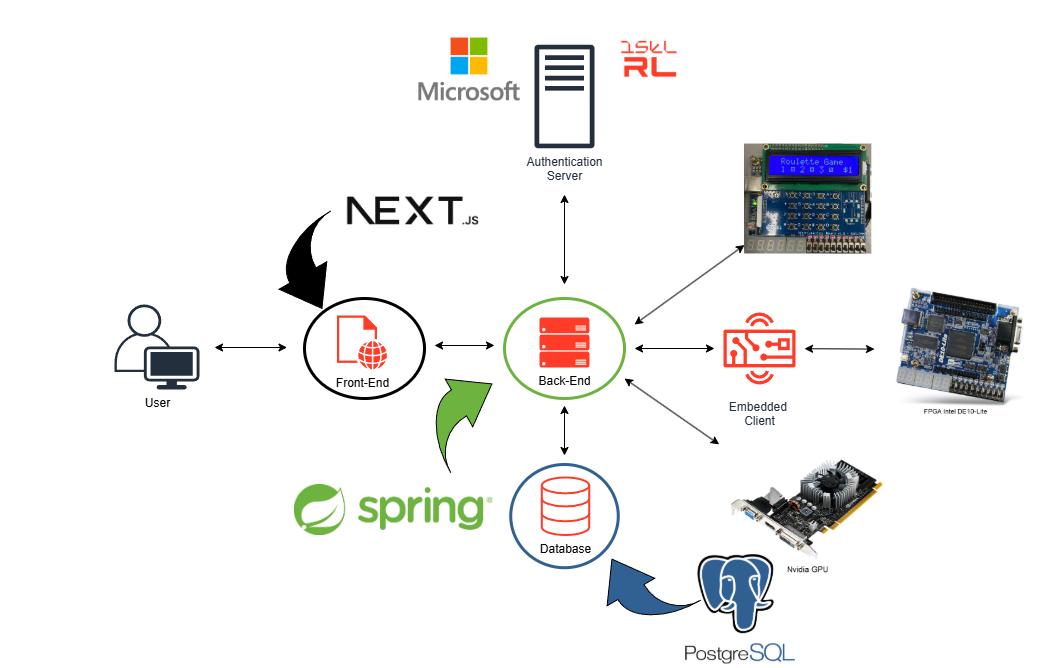
\includegraphics{../img/SystemArchitectureWithTechRL.png}}
    \end{center}
    \caption{System Architecture Overview}
    \label{fig:system-architecture}
\end{figure}

\section{Project Structure}
Project structure explaination.

\section{Implementation Details}
Project decisions.

\section{Database}
The database serves as the foundational component of the system architecture. PostgreSQL was selected as the database management system due to its reliability, open-source nature, and robust support for relational data models. This choice aligns with previous project implementations and provides the consistency and performance required for the system's operational needs.

This section presents a overview of the \ac{er model} and critical implementation details. Complete technical documentation is provided in the accompanying appendix.

\subsection{Entity-Relationship Model}

\begin{figure}[h]
    \begin{center}
        \resizebox{16cm}{!}{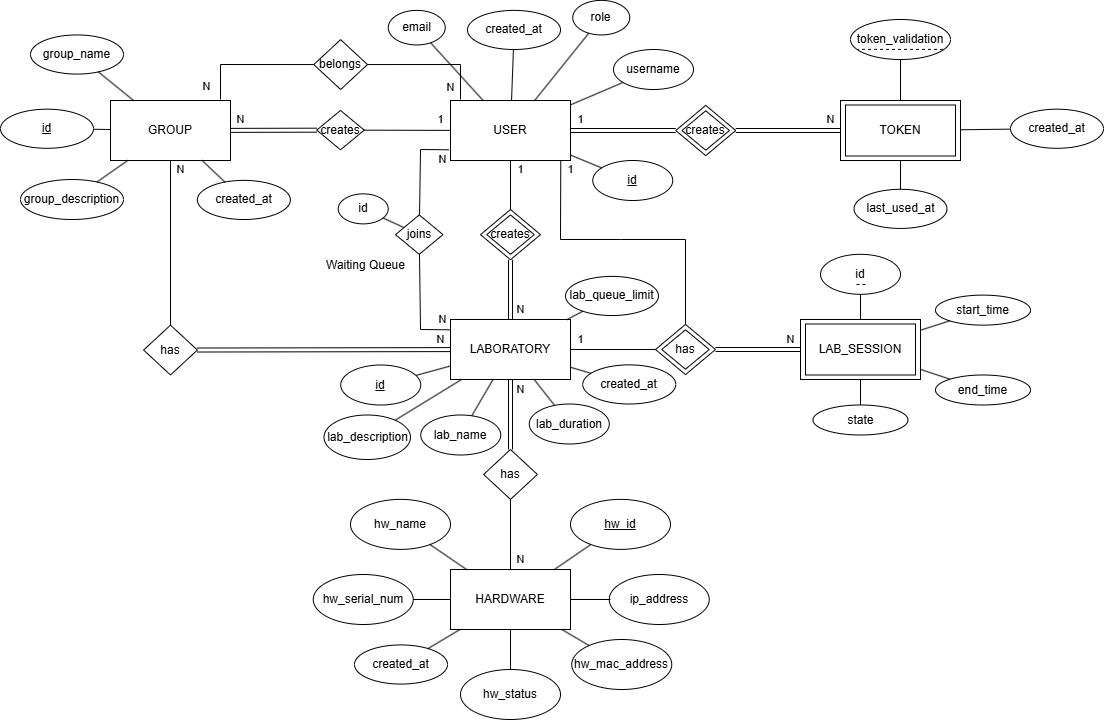
\includegraphics{../img/DB-diagrams/ERDiagramRL.drawio.png}}
    \end{center}
    \caption{Entity-Relationship Model (ER Model)}
    \label{fig:er_model}
\end{figure}

The database design follows a normalized relational structure that supports user authentication, secure session management, and the remaining system functionalities. The ER model encompasses the core entities required for system functionality while maintaining data integrity and scalability.

\subsection*{Core Entities}
\subsection*{User}

\begin{figure}[h]
    \begin{center}
        \resizebox{10cm}{!}{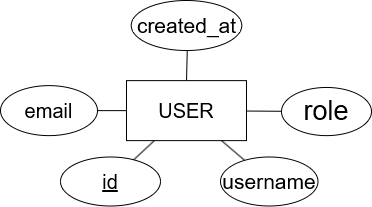
\includegraphics{../img/DB-diagrams/User.drawio.png}}
    \end{center}
    \caption{User Entity}
    \label{fig:user_entity}
\end{figure}

The \textbf{User} entity represents a user in the system. The username and email attributes are provided by the authentication system. The role serves as descriminator attribute to identify whether the user is an administrator, professor or student.

\subsection*{Token}

\begin{figure}[h]
    \begin{center}
        \resizebox{10cm}{!}{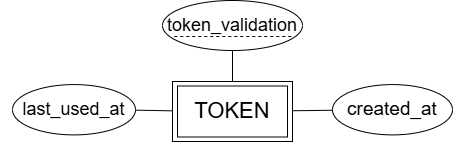
\includegraphics{../img/DB-diagrams/Token.drawio.png}}
    \end{center}
    \caption{Token Entity}
    \label{fig:token_entity}
\end{figure}

A user can create \textit{N} tokens. The \textbf{Token} is a weak entity because it cannot be identified by its attributes alone and therefore requires a user, which is a strong entity, to be identified. Its attributes cannot uniquely identify it. A token is created by only one user.

This is a useful entity for authentication propuses. It was designed to hold a hash value in the \textit{token\_validation} attribute.

Authentication workflow:

\begin{enumerate}
    \item Upon successful user login, a unique token is created with cryptographically secure values and stored in the database.
    \item For subsequent authenticated operations, the system queries the database to verify the client-provided token against stored values.
    \item Valid tokens enable secure user identification without transmitting unique identifiers.
\end{enumerate}

The \textit{last\_used\_at} and the \textit{created\_at} are useful for determining token expiration.

\subsection*{Laboratory}

\begin{figure}[h]
    \begin{center}
        \resizebox{10cm}{!}{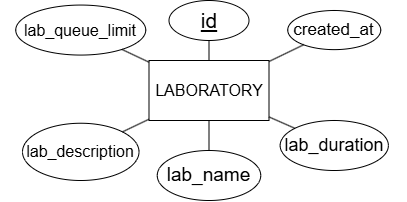
\includegraphics{../img/DB-diagrams/Laboratory.drawio.png}}
    \end{center}
    \caption{Laboratory Entity}
    \label{fig:laboratory_entity}
\end{figure}

A user, as an administrator or professor, can create \textit{N} laboratories. When creating a \textbf{Laboratory}, the user can define the name (\textit{lab\_name}) and description (\textit{lab\_description}). They can also define the duration of a laboratory session (\textit{lab\_duration}) and its queue limit (\textit{lab\_queue\_limit}).

\subsection*{Hardware}

\begin{figure}[H]
    \begin{center}
        \resizebox{10cm}{!}{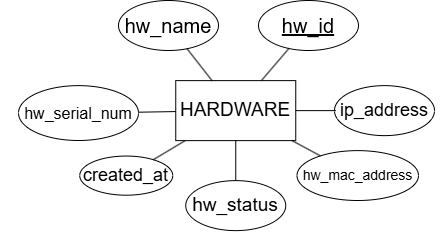
\includegraphics{../img/DB-diagrams/Hardware.drawio.png}}
    \end{center}
    \caption{Hardware Entity}
    \label{fig:hardware_entity}
\end{figure}

Upon successful laboratory creation, the user can associate \textbf{Hardware} to it, which must be created separately.

For the creation, it requires a name (\textit{hw\_name}), IP (\textit{ip\_address}) and MAC (\textit{mac\_address}) addresses (which can be null depending on the hardware), a status (\textit{hw\_status}) to indicate whether the hardware is under maintenance, occupied, or available, and a serial number (\textit{hw\_serial\_num}) to uniquely identify the hardware. Although it has an ID, the serial number helps physically identify the hardware.    

\subsection*{Group}

\begin{figure}[h]
    \begin{center}
        \resizebox{9cm}{!}{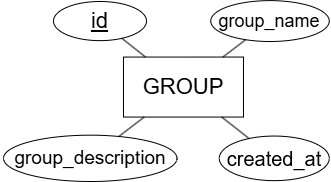
\includegraphics{../img/DB-diagrams/Group.drawio.png}}
    \end{center}
    \caption{Group Entity}
    \label{fig:group_entity}
\end{figure}

For a student to access a laboratory, they must be in a group that is associated with that laboratory. A professor can create a \textbf{Group} and associate users to it.

When creating a group, the user needs to name it (\textit{group\_name}) and, optionally, add a description (\textit{group\_description}) to it.

\subsection*{Lab Session}

\begin{figure}[H]
    \begin{center}
        \resizebox{7.5cm}{!}{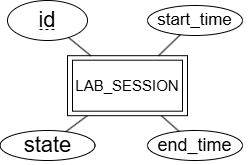
\includegraphics{../img/DB-diagrams/LabSession.drawio.png}}
    \end{center}
    \caption{Lab Session Entity}
    \label{fig:lab_session_entity}
\end{figure}

Finally, a user can join a laboratory if they are in a group associated with it. If the laboratory is being used, the user enters a waiting queue; otherwise, a \textbf{Lab Session} is created.

Lab Session is a weak entity. It requires two strong entities to be identified: the \textbf{User} entity and the \textbf{Laboratory} entity. This is used to check whether a user is in a lab session or for statistical purposes. The \textit{state} attribute indicates whether the session is over or still running. The \textit{start\_time} and \textit{end\_time} can be used for statistical details, such as determining how much time a user spent in a laboratory, or for future purposes, such as scheduling sessions.

\subsection{Implementation Details}
After providing an overview of the database entities and their associations, there are important details worth mentioning:

\begin{itemize}
    \item Although PostgreSQL is being used for its functionalities, it was decided that all logic and verifications are implemented in the Web API, so that no triggers or complex constraints are implemented on the database side.
\end{itemize}

\subsection{Conclusion}
This section has provided an overview of the database architecture, implementation, and design decisions. It has also presented the \acs{er model} of the database and described a typical user journey, explaining database interactions.

The documentation should be consulted for a comprehensive deep dive. It explains every entity, its attributes, and provides theoretical insights.

\section{Web API}
Web API

\section{Web Application}
Web App

\section{Deployment}

\section{Technologies Used}

\begin{itemize}
    \item \textbf{Frontend:} Implemented with Next.js (React framework), providing a modern, responsive web interface for users to interact with laboratories, schedule sessions, and control hardware.
    \item \textbf{Backend:} Developed in Kotlin using Spring Boot, exposing RESTful APIs for user management, authentication, laboratory session control, and business logic enforcement.
    \item \textbf{Database:} PostgreSQL is used to persist user data, session information, access logs, and configuration settings.
    \item \textbf{ORM/Database Access:} JDBI is used for type-safe, modular database access in the backend.
    \item \textbf{Authentication:} Microsoft OAuth via NextAuth is used for user authentication, supporting multiple roles (student, professor, administrator).
    \item \textbf{Containerization:} Docker is used to containerize all major components (frontend, backend, database), ensuring consistent deployment across environments.
    \item \textbf{Orchestration:} Docker Compose manages multi-container deployment, networking, and environment configuration.
\end{itemize}

\section{System Components}

\begin{itemize}
    \item \textbf{Web Application (Frontend):} Provides dashboards, laboratory access, real-time hardware monitoring, and session management. Built with Next.js and deployed as a Docker container.
    \item \textbf{API Server (Backend):} Handles authentication, authorization, laboratory and user management, and hardware abstraction. Built with Kotlin and Spring Boot, also containerized.
    \item \textbf{Database:} PostgreSQL instance running in a Docker container, with persistent storage volumes.
    \item \textbf{Hardware Abstraction Layer:} Backend modules abstract hardware-specific details, exposing unified interfaces for laboratory equipment control.
\end{itemize}

\section{Deployment Architecture}

The system is deployed using Docker Compose, which defines and manages the following services:

\begin{itemize}
    \item \textbf{db:} PostgreSQL database container, with health checks and persistent volumes.
    \item \textbf{api:} Backend API container, built from the Kotlin/Spring Boot project, depending on the database service.
    \item \textbf{website:} Frontend container, built from the Next.js project, depending on the API service.
\end{itemize}

All services are connected via Docker networks to ensure secure and efficient communication. Environment variables and secrets are managed via \texttt{.env} files.

\section{Build and CI/CD}

\begin{itemize}
    \item \textbf{Gradle:} Used for building and managing backend dependencies.
    \item \textbf{NPM:} Used for frontend dependency management and builds.
    \item \textbf{Dockerfiles:} Multi-stage builds are used for both backend and frontend to optimize image size and security.
    \item \textbf{GitHub Actions:} (If applicable) Used for continuous integration and automated builds.
\end{itemize}

\section{Notable Implementation Details}

\begin{itemize}
    \item The backend uses JDBI for database access, configured with application-specific requirements.
    \item Environment variables are used to configure database connections and secrets, improving security and flexibility.
    \item The system supports role-based access control, with different permissions for students, professors, and administrators.
    \item The hardware abstraction layer allows for future extension to new types of laboratory equipment.
\end{itemize}

\section{Summary}

The implemented infrastructure leverages modern web technologies, containerization, and modular design to provide a robust, scalable, and maintainable platform for remote laboratory access.